%META {"question":"Trong tam giác nhọn ABC, ba đường cao cắt nhau tại H. Điểm H được gọi là gì?","options":["Trực tâm của tam giác","Trọng tâm của tam giác","Tâm đường tròn ngoại tiếp","Trung điểm của cạnh BC"],"answer":0,"note":"Giao điểm của ba đường cao trong một tam giác gọi là trực tâm của tam giác đó."}
\documentclass[border=5pt]{standalone}
\usepackage{tkz-euclide}
% Màu dùng chung cho toàn bộ hình vẽ (ảnh stack với nền tối của web)
\definecolor{tminc}{RGB}{226,232,240}   % chữ + nét chính
\definecolor{tmblue}{RGB}{0,210,255}    % nhấn neon xanh
\definecolor{tmpink}{RGB}{255,0,200}    % nhấn neon hồng
\definecolor{tmgreen}{RGB}{0,255,136}   % nhấn neon xanh lá
\color{tminc}

\begin{document}
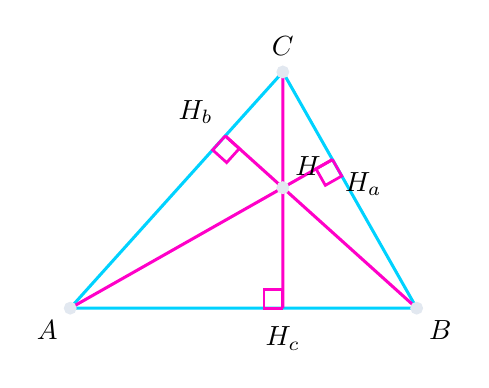
\begin{tikzpicture}[line width=1.1pt]
  \coordinate (A) at (0,0);
  \coordinate (B) at (4.4,0);
  \coordinate (C) at (2.7,3);
  \tkzDefPointBy[projection=onto B--C](A) \tkzGetPoint{Ha}
  \tkzDefPointBy[projection=onto A--C](B) \tkzGetPoint{Hb}
  \coordinate (Hc) at (2.7,0);
  \tkzInterLL(A,Ha)(B,Hb) \tkzGetPoint{H}
  \tkzDrawPolygon[tmblue,line width=1.1pt](A,B,C)
  \draw[tmpink] (A) -- (Ha) (B) -- (Hb) (C) -- (Hc);
  \tkzMarkRightAngles[size=0.24,color=tmpink,line width=1pt](B,Ha,A A,Hb,B A,Hc,C)
  \tkzDrawPoints[size=3.5,color=tminc,fill=tminc](A,B,C,H)
  \tkzLabelPoint[below left=1pt](A){$A$}
  \tkzLabelPoint[below right=1pt](B){$B$}
  \tkzLabelPoint[above=2pt](C){$C$}
  \tkzLabelPoint[above right=1pt](H){$H$}
  \tkzLabelPoint[below right=1pt](Ha){$H_a$}
  \tkzLabelPoint[above left=1pt](Hb){$H_b$}
  \tkzLabelPoint[below=3pt](Hc){$H_c$}
\end{tikzpicture}
\end{document}
